\documentclass[pra,12pt]{revtex4}
\usepackage{amsmath}
\usepackage{enumerate}
\usepackage{amssymb}
\usepackage{graphicx}
\usepackage{color}
\usepackage{mathrsfs}
\usepackage{calligra}
\usepackage[pdfborder={0 0 0},colorlinks=true,linkcolor=blue,urlcolor=blue]{hyperref}

\def\ket#1{\left|#1\right\rangle}
\def\bra#1{\left\langle#1\right|}
\def\braket#1{\left\langle#1\right\rangle}

\DeclareMathAlphabet{\mathcalligra}{T1}{calligra}{m}{n}
\DeclareFontShape{T1}{calligra}{m}{n}{<->s*[2.4]callig15}{}

\usepackage{fancyhdr}
\fancyhf{}
\lhead{\tiny Y.~D.~Chong}
\rhead{\scriptsize PH4401: Quantum Mechanics III}
\lfoot{}
\rfoot{\thepage}
\pagestyle{fancy}

\setlength{\parindent}{14pt}
\renewcommand{\theequation}{E.\arabic{equation}}
\renewcommand{\thesection}{E\arabic{section}}

\renewcommand{\baselinestretch}{1.0}
\setlength{\parskip}{0.07in}

\begin{document}

\begin{center}
{\large \textbf{Appendix F: Anyons}}
\end{center}

One of the strangest consequences of magnetic vector potentials,
introduced in Chapter 4, is that they can influence the statistics of
identical particles.  In two spatial dimensions---and \textit{only} in
2D---vector potentials can give rise to a class of identical particles
known as \textbf{anyons}, which act like neither the fermions nor
bosons discussed in Chapter 3.  Anyons have a form of particle
exchange symmetry intermediate between the fermionic and
bosonic cases.

\section{Bound Flux Tubes}

The theory of anyons created by vector potentials was developed by
\hyperref[cite:wilczek]{Wilczek (1982)}.  He considered a scenario
with set of identical particles moving in 2D (the $x$-$y$ plane), with
each particle carrying a ``flux tube'' pointing along $z$, as shown in
the figure below:

\begin{figure}[h]
  \centering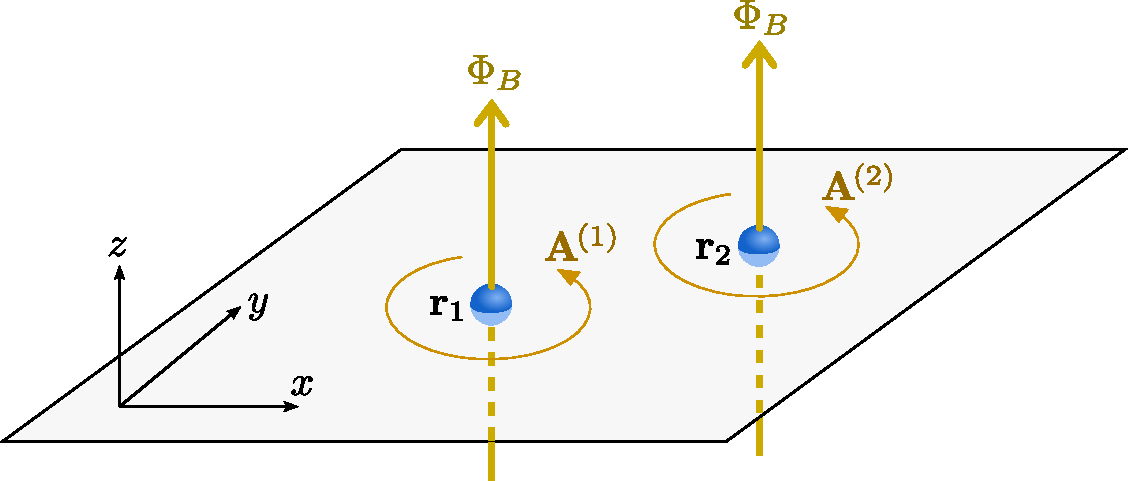
\includegraphics[width=0.7\textwidth]{anyons}
\end{figure}

Each flux tube is an infinitely thin concentration of magnetic flux
$\Phi_B$, which can be described by a singular vector potential (as
discussed in Chapter 4, Section I.C).  If $\mathbf{r}_n$ is the center
of the $n$-th particle, its vector potential is
\begin{equation}
  \mathbf{A}^{(n)}(\mathbf{r}) = \frac{\Phi_B}{2\pi
    |\mathbf{r}-\mathbf{r}_n|} \; \mathbf{e}_\phi^{(n)}(\mathbf{r}),
  \label{Asolenoid}
\end{equation}
where $\mathbf{e}_\phi^{(n)}(\mathbf{r})$ denotes the azimuthal unit
vector at position $\mathbf{r}$ relative to the origin $\mathbf{r}_n$.
The superscript $(n)$ denotes that this vector potential is centered
on the $n$-th flux tube.

Suppose the particles carrying these flux tubes also have electric
charge $-e$.  Each particle $m$ is acted upon by the vector potentials
from all the other particles, which appear in the Hamiltonian
according to the prescription
\begin{equation}
  \hat{\mathbf{p}}_m \rightarrow \hat{\mathbf{p}}_m
  + e \sum_{n \ne m} \mathbf{A}^{(n)}(\hat{\mathbf{r}}_m),
\end{equation}
where $\hat{\mathbf{p}}_m$ is the momentum operator for particle $m$.
Note that each particle's flux tube does not act upon itself (just as
in the case of electrostatic forces, the electric field generated by a
particle does not act on itself).  Thus, assuming there are no other
potentials present in the system and that the particles are
non-relativistic, the Hamiltonian is
\begin{equation}
  \hat{H} = \frac{1}{2m} \sum_m \Big| \,\hat{\mathbf{p}}_m
  + e \sum_{n \ne m} \mathbf{A}^{(n)}(\hat{\mathbf{r}}_m)\,\Big|^2.
\end{equation}

We will specifically consider the case of two particles.  In the
wavefunction representation, the Hamiltonian is
\begin{equation}
  \hat{H} = \frac{1}{2m} \left( \left| \, -i\hbar \nabla_1
  + e\mathbf{A}^{(2)}(\mathbf{r}_1)\,\right|^2
  + \left| \, -i\hbar \nabla_2
  + e\mathbf{A}^{(1)}(\mathbf{r}_2)\,\right|^2\right),
  \label{HamA}
\end{equation}
where $\nabla_m$ (for $m = 1,2$) is the gradient operator using
partial derivatives on $\mathbf{r}_m$, with the other particle
position fixed.  This Hamiltonian acts upon two-particle wavefunctions
of the form $\psi(\mathbf{r}_1, \mathbf{r}_2)$, obeying either
fermionic or bosonic exchange symmetry:
\begin{equation}
  \psi(\mathbf{r}_1, \mathbf{r}_2) = \sigma \psi(\mathbf{r}_2, \mathbf{r}_1),
  \label{exchange}
\end{equation}
where $\sigma = 1$ for bosons and $\sigma = -1$ for fermions.

\section{Gauge transformation}

In Chapter 4, we discussed the gauge symmetry of a charged particle in
an electromagnetic field.  For simplicity, take a time-independent
vector potential $\mathbf{A}$ and zero scalar potential.  Given a
single-particle wavefunction $\psi(\mathbf{r})$ describing a particle
of charge $-e$, we know that the gauge transformed wavefunction
\begin{equation}
  \psi'(\mathbf{r}) = \psi(\mathbf{r}) \,
  \exp\!\left(-\frac{ie\Lambda(\mathbf{r})}{\hbar}\right)
\end{equation}
solves the Schr\"odinger equation with the gauge transformed vector
potential
\begin{equation*}
  \mathbf{A}'(\mathbf{r}) = \mathbf{A}(\mathbf{r}) + \nabla \Lambda(\mathbf{r}).
\end{equation*}

This symmetry can be generalized to the multi-particle case.  For
two-particle Hamiltonians of the form \eqref{HamA}, one can show that
the gauge transformed two-particle wavefunction
\begin{equation}
  \psi'(\mathbf{r}_1, \mathbf{r}_2) = \psi(\mathbf{r}_1, \mathbf{r}_2)
  \, \exp\!\left(-\frac{ie\Lambda(\mathbf{r}_1, \mathbf{r}_2)}{\hbar}\right)
\end{equation}
solves the Schr\"odinger equaton for the Hamiltonian
\begin{equation}
  \hat{H}' = \frac{1}{2m} \left( \left| \, -i\hbar \nabla_1
  + e\mathbf{A}^{(2)}(\mathbf{r}_1) + e \nabla_1 \Lambda\,\right|^2
  \;+\; \left| \, -i\hbar \nabla_2
  + e\mathbf{A}^{(1)}(\mathbf{r}_2) + e \nabla_2\Lambda\,\right|^2\right).
  \label{gaugedH}
\end{equation}
The derivation for this is left for the reader to verify, and is
almost exactly the same as the single-particle derivation from Chapter
4.  The main thing to note is that $\Lambda$ is an arbitrary function
of $\mathbf{r}_1$ and $\mathbf{r}_2$; when calculating
$\nabla_1\Lambda$, the partial derivatives with respect to
$\mathbf{r}_1$ are taken with $\mathbf{r}_2$ fixed, and vice versa for
$\nabla_2\Lambda$.

We are now interested in the case where the $\mathbf{A}^{(1)}$ and
$\mathbf{A}^{(2)}$ fields in Eq.~\eqref{gaugedH} are the flux tube
potentials of Eq.~\eqref{Asolenoid}.  It turns out that such
potentials can be cancelled out, or ``gauged away'', by a certain
choice of $\Lambda(\mathbf{r}_1, \mathbf{r}_2)$.  The gauge
transformed Hamiltonian is
\begin{equation}
  \hat{H}' = - \frac{\hbar^2}{2m} \left( \nabla_1^2 + \nabla_2^2\right),
  \label{gaugedH2}
\end{equation}
which describes a pair of free particles.

\clearpage
To determine the two-particle gauge field
$\Lambda(\mathbf{r}_1,\mathbf{r}_2)$ that achieves this, let us take a
closer look at how to express the two-particle coordinates.  We can of
course write them in the Cartesian form $(x_1, y_1, x_2, y_2)$.
Alternatively, we can express them using a mix of center-of-mass
coordiantes and relative polar coordinates, $(X, Y, \mathcalligra{r},
\phi)$, as shown in this figure:

\begin{figure}[h]
  \centering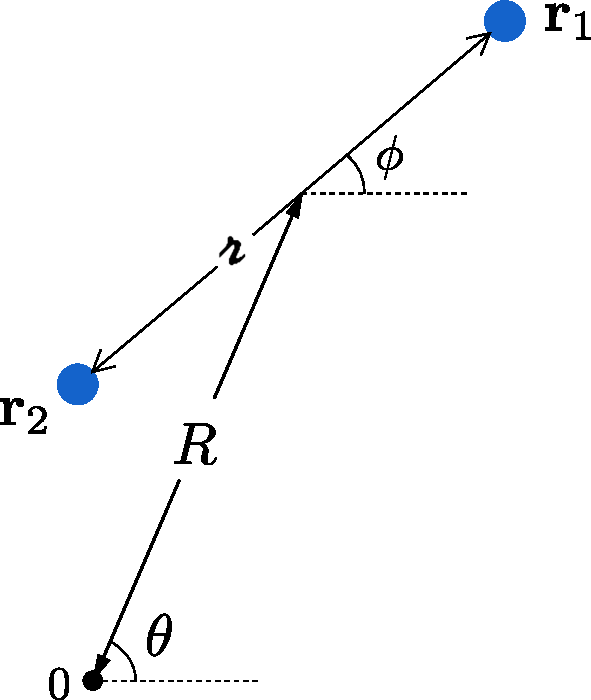
\includegraphics[width=0.27\textwidth]{anyon-coordinates}
\end{figure}

The two sets of coordinates are related by
\begin{align}
  \left\{\;
  \begin{aligned}
    X &= (x_1+x_2)/2 \\
    Y &= (y_1+y_2)/2 \\
    \mathcalligra{r} &= \sqrt{\left(x_1-x_2\right)^2 + \left(y_1-y_2\right)^2} \\
    \phi &= \tan^{-1}\left(\frac{y_1-y_2}{x_1-x_2}\right)
  \end{aligned}
  \right.
  \;\;\;\leftrightarrow\;\;\;
  \left\{ \;
  \begin{aligned}
    x_1 &= X + \frac{\mathcalligra{r}}{2} \,\cos\phi \\
    y_1 &= Y + \frac{\mathcalligra{r}}{2} \,\sin\phi \\
    x_2 &= X - \frac{\mathcalligra{r}}{2} \,\cos\phi \\
    y_2 &= Y - \frac{\mathcalligra{r}}{2} \,\sin\phi.
  \end{aligned}
  \right.
  \label{reparm}
\end{align}
Note, by the way, that this only works for 2D space.

From the right side of Eq.~\eqref{reparm}, we see that performing the
transformation $\phi \rightarrow \phi \pm \pi$, keeping $(X, Y,
\mathcalligra{r}\,)$ constant, is equivalent to exchanging
$\mathbf{r}_1 = (x_1,y_1)$ and $\mathbf{r}_2 =(x_2,y_2)$.  In other
words, the particles can be exchanged by a rotation of $\pm \pi$
around their fixed center of mass.  Eq.~\eqref{exchange} can thus be
written as
\begin{equation}
  \psi(X, Y, \mathcalligra{r}\,,\, \phi \pm \pi) \,=\, \sigma \, \psi(X,
  Y, \mathcalligra{r}\,, \phi),
\end{equation}
where $\sigma = 1$ for bosons and $\sigma = -1$ for fermions.

Now consider the gauge field
\begin{equation}
  \Lambda(X, Y, \mathcalligra{r}\,,\, \phi) = -\frac{\Phi_B \,\phi}{2\pi}.
  \label{Lambda}
\end{equation}
We claim that
\begin{align}
  \nabla_1 \Lambda &= - \mathbf{A}^{(2)}(\mathbf{r}_1) \label{nabla1} \\
  \nabla_2 \Lambda &= - \mathbf{A}^{(1)}(\mathbf{r}_2), \label{nabla2}
\end{align}
which causes these terms to exactly cancel out the vector potentials
in Eq.~\eqref{gaugedH}.  First, consider $\nabla_1\Lambda$.  The
derivatives must be evaluated with $\mathbf{r}_2$ fixed, which can be
done using the polar form of the gradient:
\begin{equation}
  \nabla_1\Lambda =  \frac{\partial
    \Lambda}{\partial \mathcalligra{r}} \, \mathbf{e}_{\mathcalligra{r}}
  + \frac{1}{\mathcalligra{r}} \,\frac{\partial \Lambda}{\partial \phi}
  \, \mathbf{e}^{(2)}_{\phi}.
\end{equation}
Here, $\mathbf{e}_{\mathcalligra{r}}$ and $\mathbf{e}^{(2)}_{\phi}$
are the radial and azimuthal unit vectors using $\mathbf{r}_2$ as the
origin.  Using Eq.~\eqref{Lambda},
\begin{equation}
  \nabla_1\Lambda = - \frac{\Phi_B}{2\pi\mathcalligra{r}} \,
  \mathbf{e}^{(2)}_{\phi} = - \mathbf{A}^{(2)}(\mathbf{r}_1).
\end{equation}
We have thus proven Eq.~\eqref{nabla1}, and Eq.~\eqref{nabla2} can be
proven similarly.  Hence, we arrive at the gauge transformed
free-particle Hamiltonian \eqref{gaugedH2}.

The gauge transformed two-particle wavefunction is
\begin{align}
  \begin{aligned}
  \psi'(X, Y, \mathcalligra{r}\,, \phi)
  &= \exp\!\left(\!-\,\frac{ie\Lambda}{\hbar}\right)\,
  \psi(X, Y, \mathcalligra{r}\,, \phi) \\
  &= e^{i \, \xi \phi}\; \psi(R, \theta, \mathcalligra{r}, \phi),
  \end{aligned}
\end{align}
where
\begin{equation}
  \xi = \frac{\Phi_B}{h/e}.
\end{equation}
The quantity $h/e$ in the denominator is the magnetic flux quantum
(see Chapter 4), so $\xi$ denotes the number of magnetic flux quanta
carried by each flux tube.  Now, when the two particles are exchanged,
\begin{align}
  \psi'(R, \theta, \mathcalligra{r}, \phi \pm \pi) &=
  e^{\pm i \, \xi} \,
  e^{i \, \xi \phi}\,
  \psi(R, \theta, \mathcalligra{r}, \phi \pm \pi) \\
  &= \sigma \,e^{\pm i \, \xi\pi}\;
  \psi'(R, \theta, \mathcalligra{r}, \phi).
\end{align}




\section*{References}

\begin{enumerate}[[1{]}]
\item F.~Wilczek, \textit{Quantum Mechanics of Fractional-Spin Particles},
  Phys.~Rev.~Lett.~\textbf{49}, 957 (1982).
  \label{cite:wilczek}
\end{enumerate}

\end{document}
